% Shared preamble for the Radioactive Signal Explorer explainers (docs/signals/*.tex).
\documentclass[11pt]{article}
\usepackage[letterpaper,margin=1in]{geometry}
\usepackage[T1]{fontenc}
\usepackage{lmodern}
\usepackage{microtype}
\usepackage{amsmath,amssymb,mathtools,bm}
\usepackage{siunitx}
\usepackage{graphicx}
\usepackage{booktabs,array,tabularx}
\usepackage{xcolor}
\usepackage{enumitem}
\usepackage{caption}
\usepackage[section]{placeins}
\usepackage[most]{tcolorbox}
\usepackage[colorlinks=true,linkcolor=blue!50!black,citecolor=blue!50!black,urlcolor=blue!50!black]{hyperref}
\usepackage[capitalise,noabbrev]{cleveref}
\sisetup{group-separator={,},group-minimum-digits=4,separate-uncertainty}
\definecolor{labblue}{HTML}{0088EE}
\definecolor{exbg}{HTML}{FFF7EC}
\definecolor{boxbg}{HTML}{EEF4FB}
\newtcolorbox{keyidea}[1][]{colback=boxbg,colframe=labblue,boxrule=0.6pt,arc=2pt,left=6pt,right=6pt,top=4pt,bottom=4pt,fonttitle=\bfseries,title={#1}}
\newtcolorbox{pitfall}[1][]{colback=red!3,colframe=red!55!black,boxrule=0.6pt,arc=2pt,left=6pt,right=6pt,top=4pt,bottom=4pt,fonttitle=\bfseries,title={#1}}
\newcounter{exercise}
\newtcolorbox{exercise}[1][]{colback=exbg,colframe=orange!70!black,boxrule=0.6pt,arc=2pt,left=6pt,right=6pt,top=4pt,bottom=4pt,fonttitle=\bfseries,
  title={Exercise~\refstepcounter{exercise}\theexercise\ifx\relax#1\relax\else\ (#1)\fi}}
\newcommand{\dd}{\mathrm{d}}
\newcommand{\keV}{\,\mathrm{keV}}
\newcommand{\MeV}{\,\mathrm{MeV}}
\newcommand{\me}{m_e c^2}
\newcommand{\nuc}[2]{${}^{#1}$#2}
\newcommand{\code}[1]{\texttt{#1}}
\newcommand{\explorer}{\href{https://dark-matter.ucr.edu/Signals.html}{Radioactive Signal Explorer}}
\newcommand{\seriesnote}{\noindent\small This note is one of five explaining the physics behind the \explorer: gamma rays, alpha decay, $(\alpha,n)$ neutrons, beta decay and Cherenkov light. Every figure was computed with the page's own code (\code{assets/signals-physics.js}); the \LaTeX{} sources and figure scripts are in \code{docs/signals/} of \url{https://github.com/UCRDarkMatter/dark-matter-lab-site}. Exercises are marked (A) analytic, (P) programming, (R) open-ended.\normalsize}

\title{$(\alpha,n)$ Neutrons:\\ Thick-Target Yields, Reaction Kinematics and the NeuCBOT Method}
\author{UCR Dark Matter Lab --- notes for graduate students}
\date{\today}
\begin{document}
\maketitle
\seriesnote

\begin{abstract}
Alphas from the uranium and thorium chains, slowing down in light-element material, occasionally induce $(\alpha,n)$ reactions. The resulting neutrons are one of the most important backgrounds for underground experiments. This note derives the thick-target yield, the neutron energy spectrum from two-body kinematics with each final state of the residual nucleus treated separately, and the NeuCBOT method that the $(\alpha,n)$ tab is built on. It ends with a detailed account of a frame mismatch in how TALYS neutron spectra are used, which makes spectra computed that way slightly too hard.
\end{abstract}
\tableofcontents

\section{The reaction}
In $(\alpha,n)$ an alpha of kinetic energy $E_\alpha$ strikes a target nucleus $T$ (mass $m_T$), producing a neutron and a residual nucleus $R$, possibly in an excited state $E_x$:
\begin{equation}
\alpha + T \to n + R^{(*)}, \qquad Q = (m_\alpha + m_T - m_n - m_R)c^2 .
\end{equation}
For the light targets that dominate in practice, $Q$ can be positive (\nuc{13}{C}: $+2.216$, \nuc{9}{Be}: $+5.70$, \nuc{17}{O}: $+0.59\MeV$) or negative (\nuc{18}{O}: $-0.70$, \nuc{19}{F}: $-1.95$, \nuc{27}{Al}: $-2.65\MeV$, \nuc{23}{Na}: $-2.97$). Even for $Q>0$ the alpha must penetrate the Coulomb barrier, so cross sections are tiny at low energy and rise steeply. Heavy targets contribute little because their barriers are too high for alphas below \SI{9}{MeV}.

\section{Thick-target yield}
An alpha emitted inside a material slows down continuously and stops; at each energy it has a chance to react. If $S(E) = -\frac{1}{\rho}\frac{\dd E}{\dd x}$ is the mass stopping power (MeV\,cm$^2$/g) and $n_i$ the number of atoms of target isotope $i$ per gram, the probability of a reaction while the alpha loses $\dd E$ is $n_i\,\sigma_i(E)\,\dd E/S(E)$. Summing over the whole slowing-down path gives the yield per alpha of initial energy $E_0$:
\begin{equation}
Y(E_0) = \sum_i n_i \int_0^{E_0} \frac{\sigma_i(E)}{S(E)}\,\dd E .
\label{eq:yield}
\end{equation}
With $\sigma$ in mb ($\SI{1e-27}{cm^2}$) this is a dimensionless number per alpha, typically \numrange{e-8}{e-5}. The stopping power of a compound follows Bragg additivity, $S = \sum_j w_j S_j$, with element tables from SRIM \cite{srim} (\code{data/signals/alpha\_stopping.json}).

\Cref{eq:yield} assumes the alpha's range is much larger than any structure in the material (a ``thick target'') and that the alpha source is uniformly mixed with the target material, so that alphas leaving one region are replaced by alphas entering from another (secular equilibrium in space). For thin coatings or surfaces you need the thin-target version, $Y = \sum_i n_i\,\sigma_i(E)\,\rho\,\Delta x$, which the explorer also offers.

\begin{keyidea}[Sanity numbers]
For acrylic (PMMA) and a \SI{5.304}{MeV} \nuc{210}{Po} alpha the explorer gives $Y = \num{1.2e-7}$ neutrons per alpha, 86\% from \nuc{13}{C} (1.1\% natural abundance) and the rest from \nuc{18}{O} and \nuc{17}{O}. A detector with \SI{1}{t} of acrylic containing \SI{1}{mBq/kg} of \nuc{210}{Po} would therefore see about $10^3\times10^{-3}\times\num{1.2e-7}\times\num{3.15e7} \approx 4$ neutrons per year from this alone.
\end{keyidea}

\section{Cross sections from TALYS}
Measured $(\alpha,n)$ cross sections exist for only a handful of targets, and very few are resolved by final state. NeuCBOT \cite{neucbot} therefore uses TALYS \cite{talys}, a Hauser--Feshbach statistical-model code, to compute for every stable isotope and every alpha energy on a \SI{0.1}{MeV} grid:
\begin{itemize}
\item the total $(\alpha,n)$ cross section $\sigma(E)$;
\item the cross section to each discrete level of the residual nucleus, $\sigma_\ell(E)$, from TALYS's level-population output;
\item the emitted-neutron energy spectrum $\dd\sigma/\dd\varepsilon$ (the ``NSpectra'' files).
\end{itemize}
\code{tools/signals/alphan.py} extracts these into one JSON file per target (\code{data/signals/alphan/}). \Cref{fig:xs} shows \nuc{13}{C}.

\begin{figure}[htbp]
\centering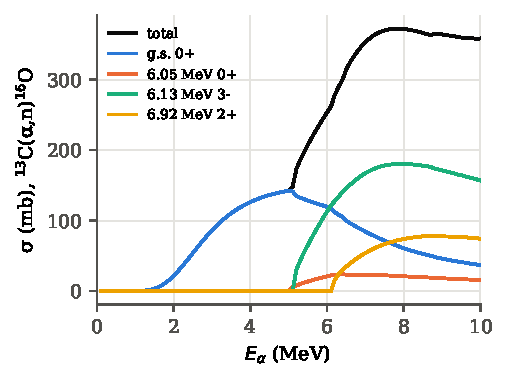
\includegraphics[width=0.62\linewidth]{fig/n_xs.pdf}
\caption{TALYS \nuc{13}{C}$(\alpha,n)$\nuc{16}{O} cross section and its split into the ground state and the first excited states of \nuc{16}{O}. Below about \SI{5}{MeV} nearly every reaction leaves \nuc{16}{O} in its ground state.}
\label{fig:xs}
\end{figure}

\begin{pitfall}[Statistical models average over resonances]
Hauser--Feshbach cross sections are energy averages. Light targets such as \nuc{13}{C} have strong, narrow resonances at low energy, so TALYS can be off by tens of per cent at a given energy; the thick-target integral \cref{eq:yield} averages much of this out, but not all. Where evaluated data exist (JENDL/AN-2005, measured thick-target yields), compare against them; tools such as SOURCES-4C, NeuCBOT and SaG4n agree on total yields to roughly 10--30\% for common materials.
\end{pitfall}

\section{Kinematics: one final state at a time}
\subsection{Centre-of-mass energies}
Non-relativistic kinematics is adequate (the alpha velocity is $\beta\approx0.05$). The kinetic energy available in the CM frame is
\begin{equation}
E_\text{cm} = E_\alpha \frac{m_T}{m_\alpha + m_T},
\end{equation}
and after the reaction the total CM kinetic energy of the outgoing pair is the \emph{channel energy}
\begin{equation}
\varepsilon = E_\text{cm} + Q - E_x .
\label{eq:channel}
\end{equation}
The neutron gets the share of $\varepsilon$ dictated by momentum balance with the residual nucleus,
\begin{equation}
E_n^\text{cm} = \frac{m_R}{m_n + m_R}\,\varepsilon .
\label{eq:encm}
\end{equation}
\subsection{Transformation to the lab}
The CM moves with velocity $V = \sqrt{2E_\alpha/m_\alpha}\;m_\alpha/(m_\alpha+m_T)$. A neutron moving with the CM would have kinetic energy $E_V = \tfrac12 m_n V^2 = m_n m_\alpha E_\alpha/(m_\alpha + m_T)^2$. Adding velocities, a neutron emitted at CM angle $\theta^*$ has
\begin{equation}
E_n = E_n^\text{cm} + E_V + 2\sqrt{E_n^\text{cm} E_V}\,\cos\theta^* .
\label{eq:lab}
\end{equation}
For isotropic emission in the CM, $\cos\theta^*$ is uniform, and since \cref{eq:lab} is linear in $\cos\theta^*$ the lab energy is \emph{uniform} between
\begin{equation}
E_n^\text{min,max} = \left(\sqrt{E_n^\text{cm}} \mp \sqrt{E_V}\right)^2 ,
\label{eq:box}
\end{equation}
with mean $E_n^\text{cm} + E_V$. (If $E_V > E_n^\text{cm}$, as near threshold for $Q<0$, all neutrons go forward and two lab energies correspond to each lab angle, but the energy distribution is still the same flat box.) In terms of the lab angle $\theta$ the familiar closed form is
\begin{equation}
\sqrt{E_n} = \frac{\sqrt{m_\alpha m_n E_\alpha}\cos\theta \pm \sqrt{m_\alpha m_n E_\alpha \cos^2\theta + (m_R + m_n)\left[m_R Q' + (m_R - m_\alpha)E_\alpha\right]}}{m_R + m_n},
\label{eq:angle}
\end{equation}
with $Q' = Q - E_x$, plotted in \cref{fig:kin}. \code{anKinematics()} implements \cref{eq:channel,eq:encm,eq:box}.

\begin{figure}[htbp]
\centering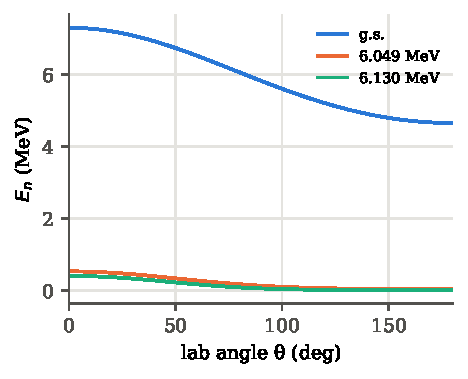
\includegraphics[width=0.62\linewidth]{fig/n_kin.pdf}
\caption{Lab neutron energy versus lab angle for \nuc{13}{C}$(\alpha,n)$\nuc{16}{O} at $E_\alpha = \SI{5.304}{MeV}$ for the ground state and the \SI{6.049}{MeV} ($0^+$) and \SI{6.130}{MeV} ($3^-$) states, from \cref{eq:angle}.}
\label{fig:kin}
\end{figure}

\subsection{The thick-target spectrum}
Combining the slowing-down integral with the kinematics, level by level:
\begin{equation}
\frac{\dd Y}{\dd E_n} = \sum_i n_i \int_0^{E_0}\frac{\dd E}{S(E)}\sum_\ell \sigma_{i\ell}(E)\;
\frac{\Theta\!\left(E_n - E_n^\text{min}\right)\Theta\!\left(E_n^\text{max} - E_n\right)}{E_n^\text{max} - E_n^\text{min}},
\label{eq:spec}
\end{equation}
with $E_n^\text{min,max}(E, \ell)$ from \cref{eq:box}. This is the solid curve in the explorer (``sum of final states, lab two-body kinematics''); each final state is also shown as a partial curve, labelled with the residual level's energy and $J^\pi$ (\cref{fig:spec}). The integral is evaluated in \SI{10}{keV} steps of alpha energy, with each box spread over the output bins in proportion to its overlap.

\begin{keyidea}[Why the final state matters beyond the spectrum]
The residual level determines the \emph{gamma} that accompanies the neutron. \nuc{13}{C}$(\alpha,n)$ to the \SI{6.130}{MeV} $3^-$ state of \nuc{16}{O} emits a \SI{6.13}{MeV} gamma; to the \SI{6.049}{MeV} $0^+$ state it emits an $e^+e^-$ pair ($0^+\to0^+$ cannot proceed by single-photon emission). These prompt signals let a detector tag $(\alpha,n)$ events, and their rates are given directly by the partial cross sections.
\end{keyidea}

\begin{figure}[htbp]
\centering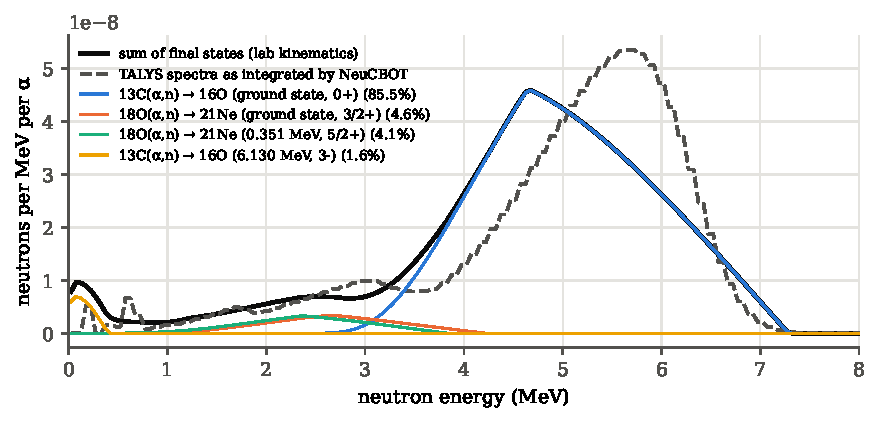
\includegraphics[width=0.72\linewidth]{fig/n_spec.pdf}
\caption{Thick-target neutron spectrum from \SI{5.304}{MeV} alphas in acrylic. Solid black: sum over final states with lab kinematics (\cref{eq:spec}); coloured: the largest final states with their share of the yield; dashed: the TALYS emitted-neutron spectra integrated as NeuCBOT does (\cref{sec:frame}). The total yields are identical; the shapes are not.}
\label{fig:spec}
\end{figure}

\begin{pitfall}[Isotropy is an approximation]
Compound-nucleus emission is symmetric about \ang{90} in the CM but not isotropic when only a few partial waves contribute, and direct reactions are forward-peaked. Anisotropy changes the \emph{shape} within each box (it is no longer flat) but not its endpoints. For a detector that surrounds the source the angle-integrated spectrum is what matters, and the effect is modest.
\end{pitfall}

\section{The NeuCBOT method and a frame mismatch}
\label{sec:frame}
\subsection{What NeuCBOT does}
NeuCBOT \cite{neucbot} computes \cref{eq:yield} exactly as above, and builds the spectrum by summing, at each alpha energy step, the TALYS emitted-neutron spectrum $\dd\sigma/\dd\varepsilon(E)$ from the NSpectra file nearest that energy, weighted by $n_i\,\dd E/S(E)$. That is, the spectrum is $\sum_i n_i\int \frac{\dd E}{S}\,\frac{\dd\sigma_i}{\dd\varepsilon}(E)$ binned in $\varepsilon$.

\subsection{What the TALYS spectrum actually is}
Comparing the TALYS NSpectra with the level cross sections shows that each discrete level appears in the spectrum as a peak at the \emph{channel energy} $\varepsilon = E_\text{cm} + Q - E_x$ of \cref{eq:channel}, smeared with the code's default \SI{0.2}{MeV} broadening---not at the neutron's CM energy (\cref{eq:encm}) and not at its lab energy (\cref{eq:lab}). The emission energy in a Hauser--Feshbach calculation is naturally the relative-motion energy of the outgoing channel, and for heavy residual nuclei the distinction is irrelevant because $m_R/(m_n+m_R)\to1$ and $E_V\to0$. For light targets it is not:
\begin{equation}
\langle E_n^\text{lab}\rangle = \frac{m_R}{m_n + m_R}\,\varepsilon + E_V \;<\; \varepsilon .
\end{equation}
For \nuc{13}{C}$(\alpha,n)$\nuc{16}{O} at \SI{5.3}{MeV} the factor is $16/17$ and $E_V = \SI{0.07}{MeV}$, so the TALYS peak sits about \SI{0.3}{MeV} (6\%) above the mean lab energy, and the kinematic box (here \SI{\approx 2.6}{MeV} wide, \cref{fig:kin}) is replaced by a \SI{0.2}{MeV} Gaussian.

\subsection{Consequences}
\begin{itemize}
\item \textbf{Yields are unaffected}: the total cross section is used for the yield.
\item \textbf{Spectra are too hard by 3--7\% for light targets.} For acrylic and \nuc{210}{Po} alphas the mean neutron energy is \SI{4.93}{MeV} from the TALYS spectra versus \SI{4.61}{MeV} from \cref{eq:spec}; for PTFE (\nuc{19}{F}, $m_R/(m_n+m_R) = 22/23$) it is 1.33 versus \SI{1.29}{MeV}.
\item \textbf{Kinematic broadening is missing}: lines that should be boxes several MeV wide appear as narrow peaks, which matters for anything that depends on the spectral shape (moderation, capture-gamma timing, nuclear-recoil spectra).
\item \textbf{Normalisation at single energies}: the integral of an NSpectra file divided by the TALYS total $(\alpha,n)$ cross section at the same energy ranges from 0.64 to 1.30 across the targets checked, so the raw spectra do not integrate to the yield bin by bin. The explorer's dashed curve renormalises each spectrum to $\sigma(E)$ (\code{alphaNSpectrum} also accepts \code{rawTalys: true} to integrate them unnormalised, as NeuCBOT does).
\end{itemize}
The explorer's fix is to use the level-resolved cross sections with two-body lab kinematics (\cref{eq:spec}). This covers the discrete levels only; a complete fix would also transform any continuum part of the TALYS spectrum (higher excitation energies) from the channel energy to the lab, using \cref{eq:encm} and the boost averaged over angles. For the light targets and $E_\alpha < \SI{9}{MeV}$ that dominate underground backgrounds, essentially all of the yield goes to discrete levels, so the omission is small; for heavier targets, where the continuum matters, the frame difference is itself small.


\section{Related signals}
\subsection{Spontaneous fission}
\nuc{238}{U} also fissions spontaneously (branch $5.5\times10^{-7}$), emitting $\bar\nu = 2.01$ neutrons per fission with a Watt spectrum
\begin{equation}
\chi(E) \propto e^{-E/a}\sinh\sqrt{bE},\qquad \langle E\rangle = \tfrac32 a + \tfrac14 a^2 b,
\end{equation}
($a = \SI{0.6483}{MeV}$, $b = \SI{6.811}{MeV^{-1}}$ \cite{sources4}). Per decay of the \nuc{238}{U} chain in secular equilibrium this is $1.1\times10^{-6}$ neutrons, comparable to the $(\alpha,n)$ yield in many low-$Z$ materials. The neutrons come in bursts; the multiplicity follows Terrell's Gaussian with $\sigma \approx 1.08$ \cite{terrell}, so a capture-tagging veto sees several neutrons at once.

\subsection{Prompt gammas and other channels}
Most $(\alpha,n)$ reactions leave the residual nucleus excited, and its de-excitation gammas accompany the neutron: the \SI{6.13}{MeV} gamma (and the \SI{6.05}{MeV} $0^+\to0^+$ E0 pair) from \nuc{13}{C}$(\alpha,n)$\nuc{16}{O}, or the \SI{583}{keV} and \SI{891}{keV} lines from \nuc{19}{F}$(\alpha,n)$\nuc{22}{Na} (whose ground state is itself a $\beta^+$ emitter, giving a delayed \SI{1275}{keV} gamma). Their yields follow from the same thick-target integral with the TALYS gamma-production cross sections in place of $\sigma_n$. The tab applies the same integral to the $(\alpha,p)$ and $(\alpha,\gamma)$ residual-production cross sections.

\subsection{Layers}
When the emitter sits in a layer of thickness $t$ on a backing, an alpha emitted at depth $z$ toward the backing reaches it with energy $E\big(R(E_0) - (t-z)/\cos\theta\big)$ and continues its thick-target yield in the backing's material. The layer then sees only the part of each track inside it: $Y_\text{layer} = Y(E_0) - Y(E_\text{exit})$.

\subsection{Checking the cross sections}
TALYS is a statistical-model code and can be off by tens of percent for light targets. You can upload a measured or evaluated $\sigma(E)$ (e.g.\ JENDL/AN-2005 or EXFOR) to compare. The tab recomputes that isotope's thick-target yield with your cross section and shows the ratio to TALYS.
\section{What the $(\alpha,n)$ tab outputs}
Choose a material (preset compositions or a custom element list), and either an alpha energy or an emitter (whose alpha lines are used with their intensities, or a whole chain in equilibrium). The tab returns the yield per alpha and per decay, the per-target contributions, the spectrum of \cref{eq:spec} with its final-state partials, the TALYS/NeuCBOT spectrum for comparison, the formula, and a CSV.

\section{Exercises}
\begin{exercise}[A]
Derive \cref{eq:lab,eq:box} from velocity addition, and show that the mean lab energy for isotropic CM emission is $E_n^\text{cm} + E_V$. Then derive \cref{eq:angle} directly from momentum conservation in the lab.
\end{exercise}
\begin{exercise}[A]
For \nuc{18}{O}$(\alpha,n)$\nuc{21}{Ne} ($Q = -0.70\MeV$), find the threshold alpha energy, and show that just above threshold all neutrons are emitted in a forward cone. What is the cone's half-angle as a function of $E_\alpha$?
\end{exercise}
\begin{exercise}[A]
Estimate the range of a \SI{5.3}{MeV} alpha in acrylic from the stopping powers in \code{alpha\_stopping.json}. A \nuc{210}{Po} contamination sits in a \SI{1}{\micro m} surface layer of acrylic, half of the alphas going inward. Estimate the yield per decay and compare with the bulk value.
\end{exercise}
\begin{exercise}[P]
Implement \cref{eq:yield,eq:spec} for PTFE using the JSON files in \code{data/signals/alphan/} and reproduce the solid curve of the explorer. Then build the spectrum the NeuCBOT way from the \code{nspec} arrays and verify the 1.33 vs \SI{1.29}{MeV} means quoted above.
\end{exercise}
\begin{exercise}[P]
Compute the yield of the full \nuc{238}{U} chain in secular equilibrium in borosilicate glass. Which isotopes dominate? How much does the answer change if the chain is broken at \nuc{226}{Ra} (only the upper chain present)?
\end{exercise}
\begin{exercise}[R]
A neutron veto tags $(\alpha,n)$ events by the accompanying gamma. Using the partial cross sections, estimate what fraction of acrylic $(\alpha,n)$ neutrons from \nuc{210}{Po} come with a prompt gamma or pair, and discuss what this implies for vetoing \nuc{13}{C}$(\alpha,n)$ compared with \nuc{19}{F}$(\alpha,n)$.
\end{exercise}

\begin{thebibliography}{9}
\bibitem{neucbot} S.~Westerdale and P.~D. Meyers, ``Radiogenic neutron yield calculations for low-background experiments'', Nucl.\ Instrum.\ Meth.\ A \textbf{875}, 57 (2017); NeuCBOT, \url{https://neucbot.ucr.edu}.
\bibitem{talys} A.~J. Koning, S.~Hilaire and S.~Goriely, ``TALYS: modeling of nuclear reactions'', Eur.\ Phys.\ J.\ A \textbf{59}, 131 (2023).
\bibitem{srim} J.~F. Ziegler, M.~D. Ziegler and J.~P. Biersack, ``SRIM -- The stopping and range of ions in matter'', Nucl.\ Instrum.\ Meth.\ B \textbf{268}, 1818 (2010).
\bibitem{jendl} T.~Murata, H.~Matsunobu and K.~Shibata, ``Evaluation of the $(\alpha,xn)$ reaction data for JENDL/AN-2005'', JAEA-Research 2006-052 (2006).
\bibitem{sag4n} E.~Mendoza \emph{et al.}, ``Neutron production induced by $\alpha$-decay with Geant4'', Nucl.\ Instrum.\ Meth.\ A \textbf{960}, 163659 (2020).
\bibitem{sources4} W.~B. Wilson \emph{et al.}, \emph{SOURCES 4A}, LA-13639-MS (1999); Watt parameters as used in MCNP and Geant4.
\bibitem{terrell} J.~Terrell, ``Distributions of fission neutron numbers'', Phys.\ Rev.\ \textbf{108}, 783 (1957).
\end{thebibliography}
\end{document}
